\section{Experimental Results}\label{section:experiments-results}

\subsection{Quantitative Results}\label{subsec:quantitative}

As discussed in the previous session, the four NEAT variants were
compared in two ways: First we perform three full evolution runs for
each variant/matchup pairing, and then the five best genomes obtained
from this training are run 50 times to evaluate their victory and
survival ratios. A summary of these results is presented in
Table~\ref{table:quantitative}.

\begin{table}
    \caption{Victory Ratio and Median Survival for the best genomes.
            Survival values only consider victory matches.}
    \label{table:quantitative}
    \begin{tabular}{llll}
        \toprule
        Variant & Matchup & Win Ratio & Survival \\
        \midrule
        Vanilla & marine/marine & 0.77 & 8 \\
        Unified & marine/marine & 0.77 & 8 \\
        Cascade & marine/marine & 0.85 & 8 \\
        Novelty & marine/marine & 0.55 & 8 \\[1ex]

        Vanilla & marine/zergling & 0.03 & 4 \\
        Unified & marine/zergling & 0.01 & 10 \\
        Cascade & marine/zergling & 0.05 & 5 \\
        Novelty & marine/zergling & 0.09 & 10 \\[1ex]

        Vanilla & vulture/vulture & 0.92 & 8 \\
        Unified & vulture/vulture & 0.90 & 10 \\
        Cascade & vulture/vulture & 0.93 & 8 \\
        Novelty & vulture/vulture & 0.93 & 9 \\[1ex]

        Vanilla & vulture/zealot & 0.87 & 8 \\
        Unified & vulture/zealot & 0.93 & 9 \\
        Cascade & vulture/zealot & 0.92 & 9 \\
        Novelty & vulture/zealot & 0.99 & 9 \\
        \bottomrule
    \end{tabular}
\end{table}

% \subsubsection{Victory Rate Analysis}

From this table, we can observe that in general the methods managed to
learn a good tactic to defeat their enemies, with the exception of the
marine/zergling matchup.
%\footnote{This could be considered scientific evidence that Blizzard needs to nerf zerglings}
Small variations are observed on the methods within each matchup, but
an ANOVA test confirms that these variations are not significative (F
= 0.85).

% \subsubsection{Survival Rate Analysis}

In the same fashion, it was not possible to observe a clear difference
among the variants in terms of the median number of survivors in
winning matches. Figure~\ref{fig:survivors} shows the survivor numbers
for each variation/matching pairing.

\begin{figure}
  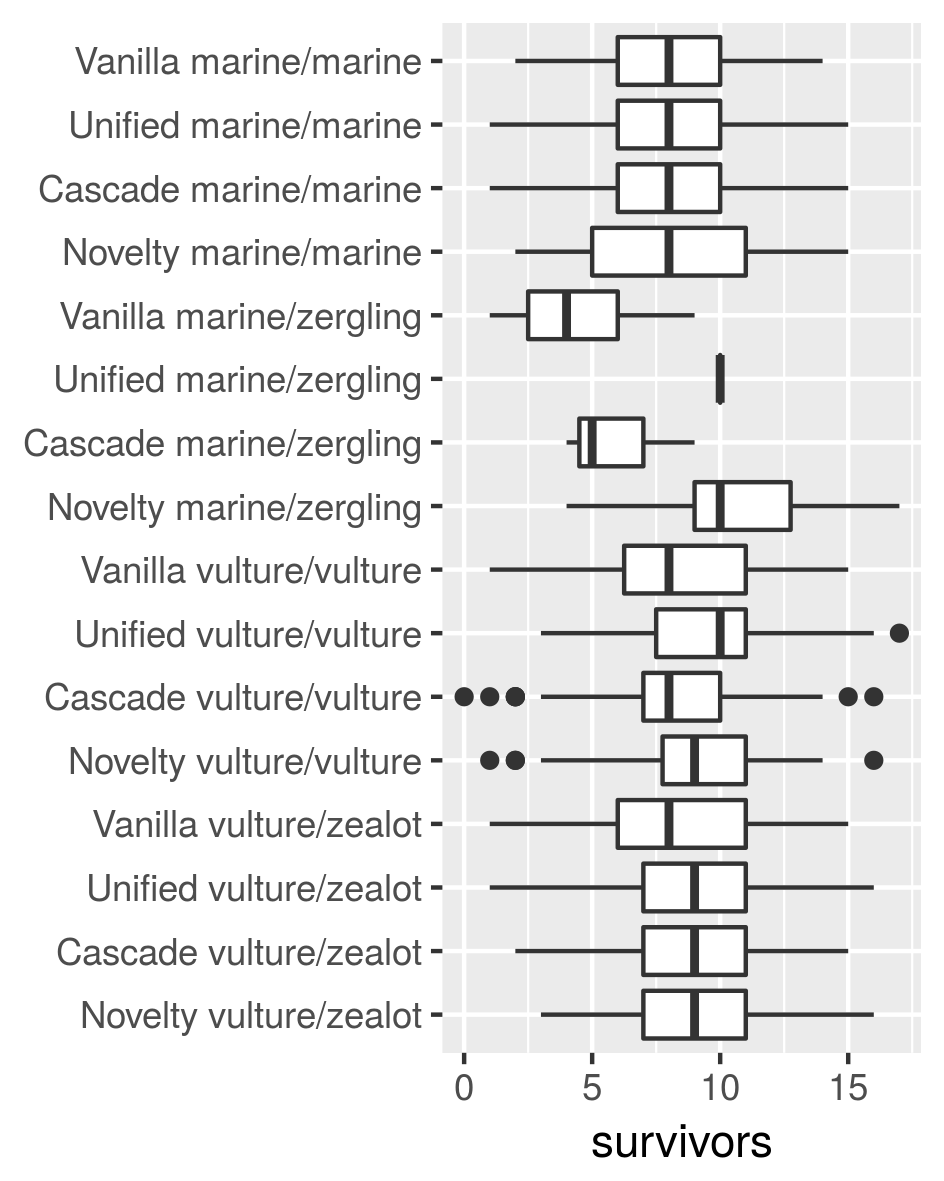
\includegraphics[width=.5\textwidth]{figures/survivors}
  \caption{Box plot for the survival ratios}\label{fig:survivors}
\end{figure}

% \subsubsection{Evolution Rate Analysis}


\begin{figure*}
  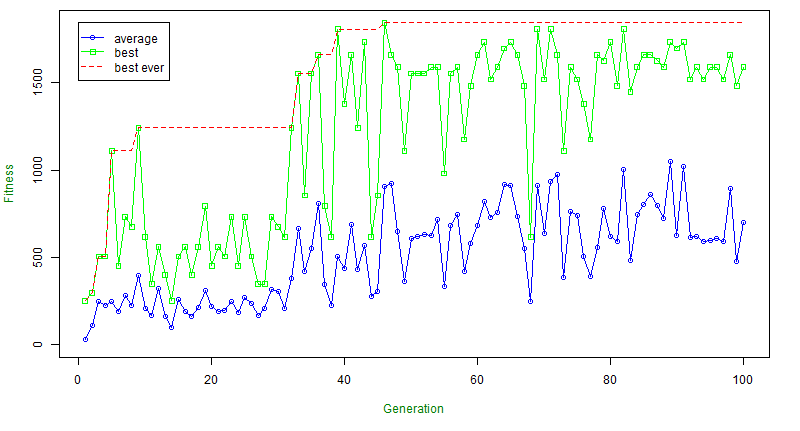
\includegraphics[width=.4\textwidth]{figures/evolution_zealot}
  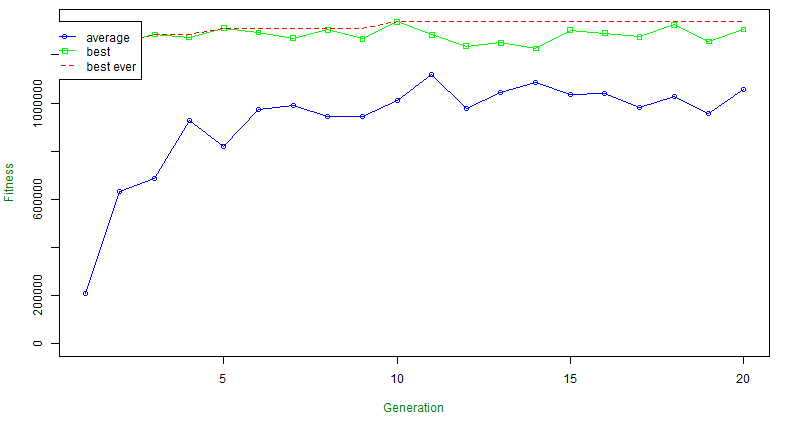
\includegraphics[width=.4\textwidth]{figures/evolution_unified}
  \caption{Training progress for two vulture vs zealot matchups. Left:
    Cascade NEAT vs zealots. Right: Unified NEAT. Note that the
    fitness function are different so absolute values should not be
    compared directly.}\label{fig:evolution}
\end{figure*}

Finally, we observed the training progress of the
experiment. Figure~\ref{fig:evolution} show two examples of training
graphs that are representative of the experiment as a
whole\footnote{the figures for all matchings can be found at the
online repository}. In the Cascade NEAT training (left side) we see
that while there is a small increase in best and mean fitness, there
are large variations every generation. In the Unified NEAT training
(right side) these variations are not present. In unified neat, all
networks in the same combat experiment share the same fitness result,
while in the other variants (such as the Cascade Neat) each network in
the same combat is evaluated separately, even though they influence
each other (a weak network will make the overall combat harder for a
stronger network).

However, while this difference is observable in the training curve, as
we see in Figure~\ref{fig:evolution}, it did not generate an
observable difference in the final result
(Table~\ref{table:quantitative}), which is interesting.

\subsection{Qualitative analysis}

From the quantitative analysis we learned that a winning strategy was
generally found (high winning ratio), while the differences among
variants was not strong. In particular, the survivor rate was the same
across methods with the exception of the particularly hard
marine/zergling matchup.

To better understand this lack of difference, and what could be done
to increase the survival ratio, we performed a qualitative analysis of the
results of the experiment by studying the different behaviors that emerged.

\subsubsection{Developping stimpack behaviour}

% TODO: add an image?

Vanilla NEAT doesn’t seems to be good a developing the stimpack behaviour since organisms
that survives without stimpack get better reward,
even though they may have survived because others used stimpacks to get in the frontline
and got themselves killed first.
So, organisms tends to lose this behaviour over generations.

CHECK: Cascade-NEAT and Novelty [expected to be approximately identical].

In comparison, the unified version, which is good a developing uniform behaviours
was somewhat better at developing this behaviour.
Indeed, since every agents use the same type of neural network, all units in the round
has the behaviour encoded and don’t win because others
did all the hard stuff.

Sadly the marines vs marines problem can be solved efficiently just by waiting for the
enemy and attacking all out mostly without stimpacks.
Depending on the enemy’s formation at it’s arrival it can be even more effective.
They can indeed shoot first with more firepower.

Novelty search got a significantly better result on the marines vs zergs experiments,
meaning it was able to develop some stimpack behaviours. [need more behaviour analysis]

Conclusion: not a big success. Overall failure.

\subsubsection{Kiting behaviour}

\begin{figure}
    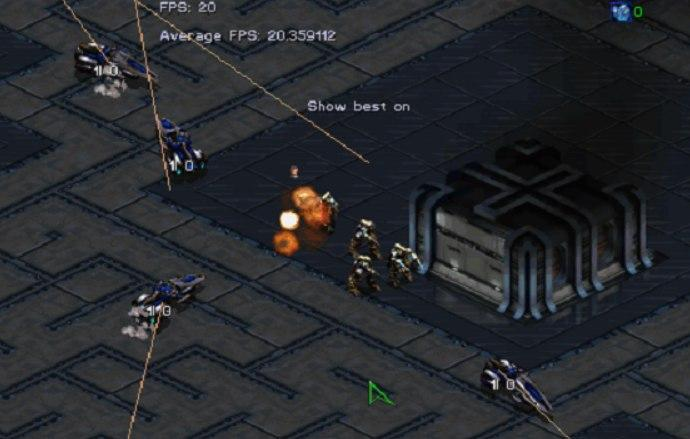
\includegraphics[width=.5\textwidth]{figures/vultures_kiting_screenshot}
    \caption{Vultures using kiting technique to beat xealots}\label{fig:vultures_kiting}
\end{figure}

All the presented method performs exceedingly well on the kiting problem (that is vultures vs zealots).
This is confirmed by the statistical results shown in subsection~\ref{subsec:quantitative}. After a short amount of generations, adequate
individuals start to emerge (even with the first species, meaning the topology required isn’t complex at all)
and after a few more generations, networks weights are tweaked to get a quite decent kiting behaviour with any
technique, the vulture is able to maintain a good distance between itself and the enemies as shown on
Figure~\ref{fig:vultures_kiting}. In some cases, vultures are even able to shoot without
losing speed and thus withdraw really quickly from risks. This ressemble
a classical vulture micro technique called “patrol micro” involving the use of the so-called patrol command's
lack of cooldown to have the vulture move, fire, and retreat without slowing down. We don’t really know how it
is achieved here without the patrol command, but it is effectively the same result.

It is interesting to note that for the matchup vultures vs vultures, our bot was even more effective by avoiding opponent's
projectiles using, again, effective kiting. Even against a ranged opponent it can shines (though here the projectives have
some physical properties unlike marines's bullets).

To improve: friendly collisions blocking effective retreat.

\subsubsection{Others}

…

